\documentclass[letterpaper,12pt]{article}
\usepackage{amsmath}  % improve math presentation
\usepackage{graphicx} % takes care of graphic including machinery
\usepackage{mathrsfs}


\usepackage[final]{hyperref} % adds hyper links inside the generated pdf file
\hypersetup{
	colorlinks=true,       % false: boxed links; true: colored links
	linkcolor=blue,        % color of internal links
	citecolor=blue,        % color of links to bibliography
	filecolor=magenta,     % color of file links
	urlcolor=blue         
}

\title{Final Project for Computational Physics}
\date{\today}
\author{Xinyu Liu}



\begin{document}
\maketitle

\begin{abstract}
    This is a code to simulate the 2D ising model under certain temperature. The basic idea for studying a thermal system is to investigate the partition function by computational method. In a word, we can choose a ensemble of states by computers, attributing each state with a boltzman probability and sum over all the state to calculate the expectation energy for the system under a certain temperature. However, a random sampling is highly uneffective for low temperature physics, since most possible states are irrelavant in low temperature. The way to carry out an more effective sampling method is by using Metropolis Algorithm, which is introduced in detail in Newman Chapter 10.3. In this work, we utilize Metropolis Algorithm to study a 2D spin system with 2D exchanging interaction and external field.
\end{abstract}

\tableofcontents



\newpage

\section{My Github Page URL}
\url{https://github.com/rising1227/phys-ga2000}

\section{Physics Model}

We investigate the physics with simplist exchange Ising interaction with an external field:

\begin{equation}
    H = \sum_{\langle i,j \rangle} -J (S_i S_j+1) + B_{k} S_k
\end{equation}

Here the index i,j,k denote the label of particular spin in the spin lattice. We modified it a bit such that the ground state of the system has zero energy(without magnetic field). $B_{k}$ denotes an external field and $\langle i,j \rangle$ denotes neighbouring pairs of spins. $B_{k}$ denotes an external field. First of all, we carry out the simulation with no external field, i.e. $B=0$, then we study this model with constant external field $B_{k} = B_0$. Finally, we investigate the system with spatially varying field $B_k$.


\section{Structure of the Code}

In order to make the code clear and make it easier for collaboration, we divide our code into different blocks. Each account for a specific purpose.

\begin{itemize}
    \item The physical system is represented by a M*M numpy array. Each spin is represented by a bool type variable. This is the most compact variable to represent a spin. We use True to represent spin up$\uparrow$ and False to represent spin down$\downarrow$. We denote our matrice as S. We also use a function to generate a initial spin array $S_0$
    \item A external magnetic field is denoted by a M*M numpy array B. $B[i][j]$ represent the external magnetic field at each point. The total energy of initial system can be calculated.
    \item A energy calculation function take S and B as input and calculate the total energy.
    \item A transfer function "Trans" is one step in the markov chain in the Metropolis method. It takes S, B, Total magnetization M, total energy E and temperature T as the input. It changes the S internally, while outputing a renewed M and E.
    \item Then we define a Metropolis function "Metro" which takes "Trans" function as an input. Also inputing the temperature T, S, B, M, E. This metropolis function reiterates the transfer function for many times and detect whether our system goes to thermal equilibrium. After thermal equilibrium, it outputs a averaged total energy and magnetization at a certain temperature.
    \item At main function, we utilize this metropolis function many times for different temperature. Finally, we can have a full curve of E and M as a function of temperature.
\end{itemize}



% \begin{table}[!h]
%     \centering
%     \caption{Dow jones(original and 2\% smoothed) industrial index over time}
%     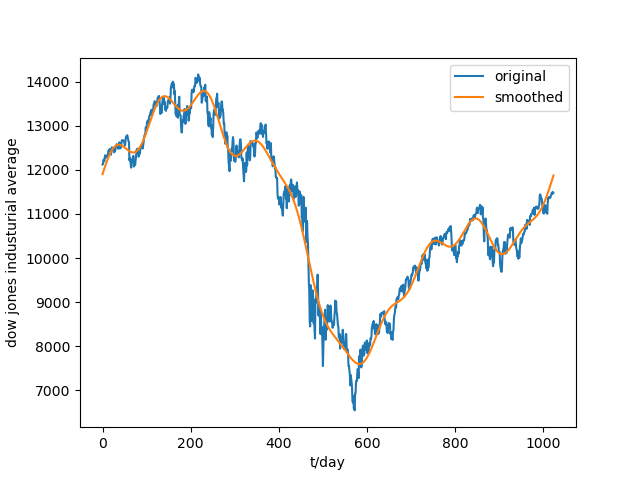
\includegraphics[width=11cm]{8-3-3.png}
% \end{table}%




\end{document}




